\documentclass[tikz,border=12pt]{standalone}
\usepackage[T1]{fontenc}
\usepackage{lmodern,amsmath,amssymb}
\usetikzlibrary{arrows.meta,positioning}
\definecolor{ink}{HTML}{183444}
\definecolor{blue}{HTML}{1B6780}
\definecolor{amber}{HTML}{AD601A}
\begin{document}
\hyphenpenalty=10000\exhyphenpenalty=10000
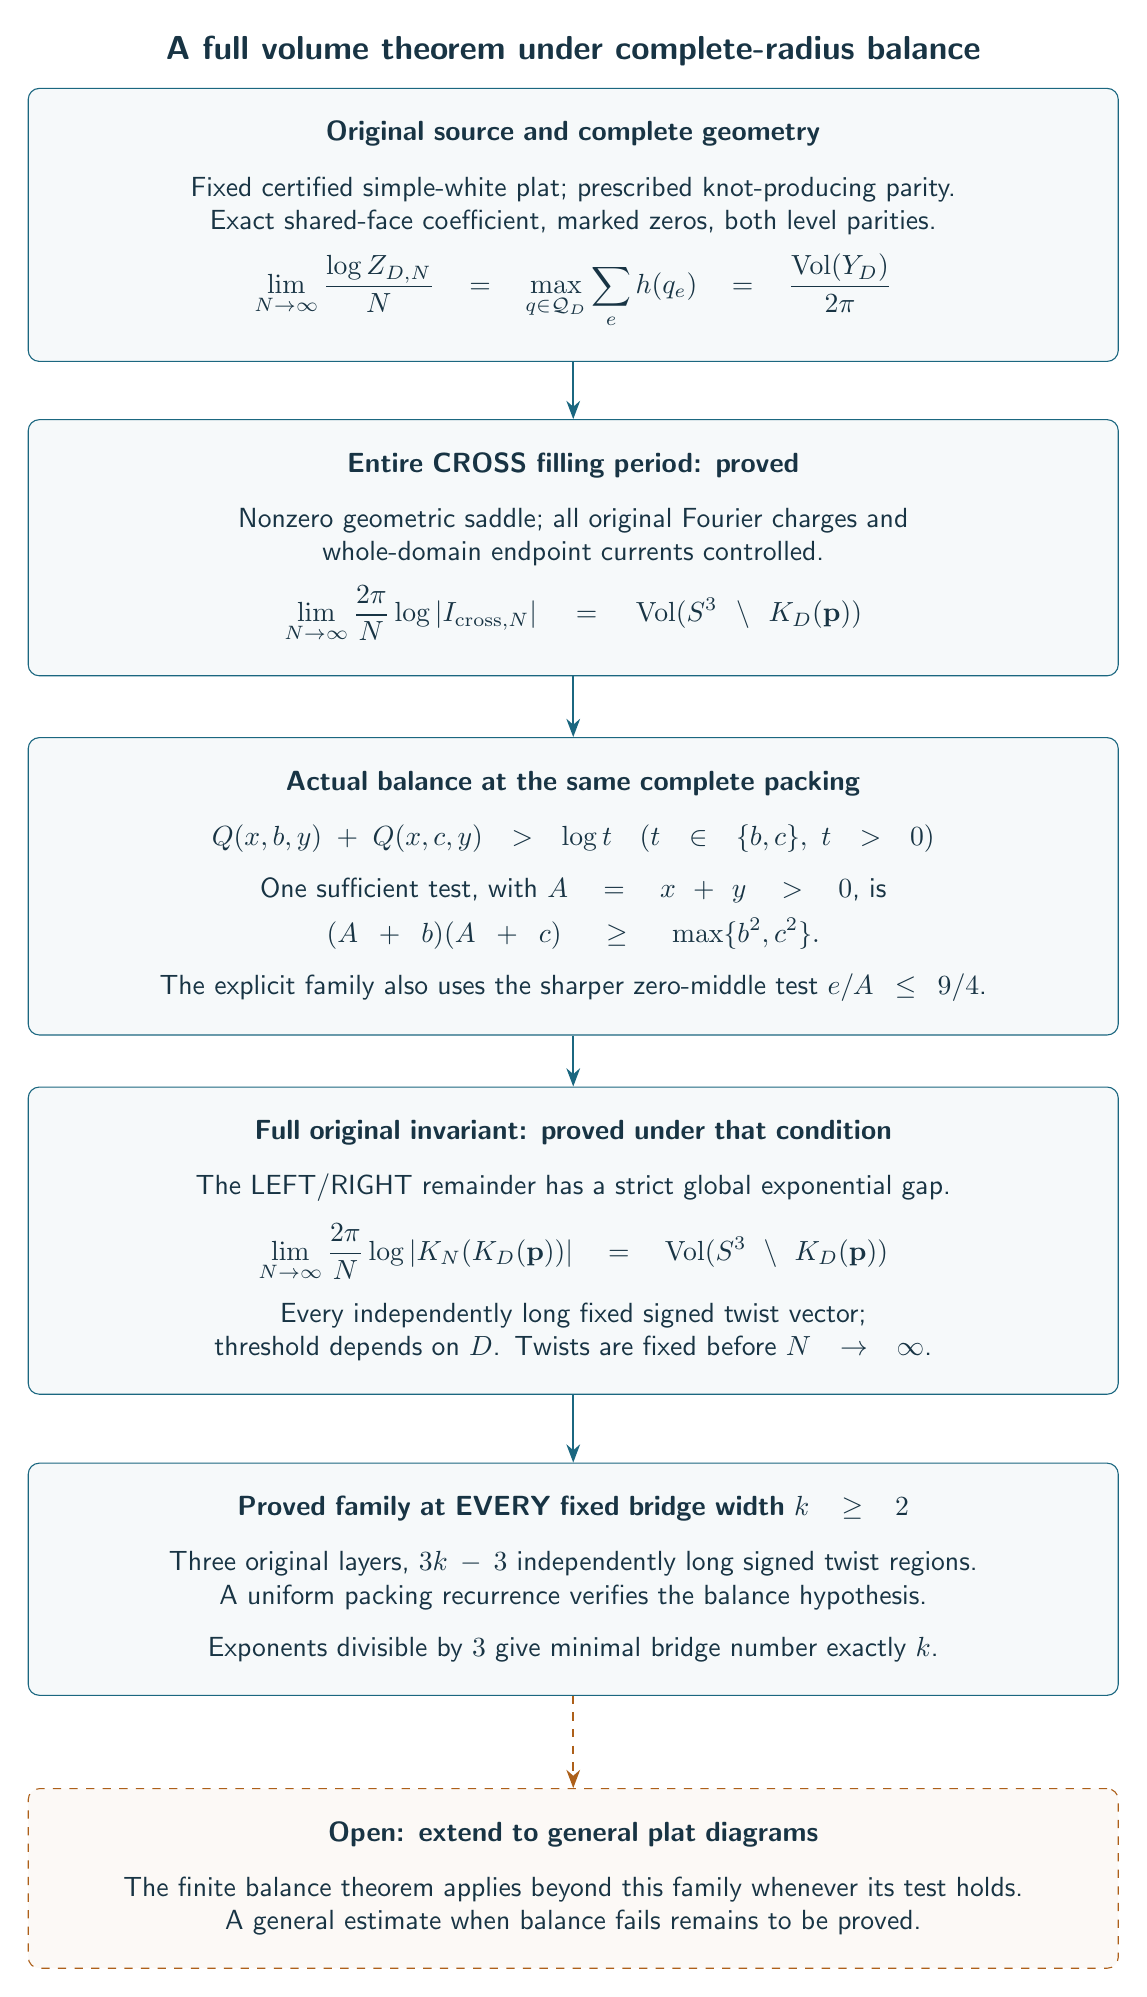
\begin{tikzpicture}[font=\sffamily,text=ink,>=Stealth,
 panel/.style={draw=blue,fill=blue!4,rounded corners,align=center,inner sep=12pt,text width=13cm},
 pending/.style={panel,draw=amber,fill=amber!4,dashed}]
 \node[font=\sffamily\large\bfseries] at (0,2.2)
 {A full volume theorem under complete-radius balance};
 \node[panel] (source) at (0,0)
 {\textbf{Original source and complete geometry}\\[8pt]
 Fixed certified simple-white plat; prescribed knot-producing parity.\\
 Exact shared-face coefficient, marked zeros, both level parities.\\[6pt]
 $\displaystyle \lim_{N\to\infty}\frac{\log Z_{D,N}}{N}
 =\max_{q\in\mathcal Q_D}\sum_e h(q_e)
 =\frac{\operatorname{Vol}(Y_D)}{2\pi}$};
 \node[panel] (cross) at (0,-4.1)
 {\textbf{Entire CROSS filling period: proved}\\[8pt]
 Nonzero geometric saddle; all original Fourier charges and\\
 whole-domain endpoint currents controlled.\\[6pt]
 $\displaystyle \lim_{N\to\infty}\frac{2\pi}{N}\log|I_{\mathrm{cross},N}|
 =\operatorname{Vol}(S^3\setminus K_D(\mathbf p))$};
 \draw[->,blue,thick] (source)--(cross);
 \node[panel] (balance) at (0,-8.4)
 {\textbf{Actual balance at the same complete packing}\\[8pt]
 $\displaystyle Q(x,b,y)+Q(x,c,y)>\log t\quad(t\in\{b,c\},\ t>0)$\\[7pt]
 One sufficient test, with $A=x+y>0$, is\\[4pt]
 $\displaystyle (A+b)(A+c)\geq\max\{b^2,c^2\}.$\\[7pt]
 The explicit family also uses the sharper zero-middle test $e/A\leq9/4$.};
 \draw[->,blue,thick] (cross)--(balance);
 \node[panel] (full) at (0,-12.9)
 {\textbf{Full original invariant: proved under that condition}\\[8pt]
 The LEFT/RIGHT remainder has a strict global exponential gap.\\[7pt]
 $\displaystyle \lim_{N\to\infty}\frac{2\pi}{N}\log|K_N(K_D(\mathbf p))|
 =\operatorname{Vol}(S^3\setminus K_D(\mathbf p))$\\[7pt]
 Every independently long fixed signed twist vector;\\
 threshold depends on $D$. Twists are fixed before $N\to\infty$.};
 \draw[->,blue,thick] (balance)--(full);
 \node[panel] (family) at (0,-17.2)
 {\textbf{Proved family at EVERY fixed bridge width $k\geq2$}\\[8pt]
 Three original layers, $3k-3$ independently long signed twist regions.\\
 A uniform packing recurrence verifies the balance hypothesis.\\[7pt]
 Exponents divisible by $3$ give minimal bridge number exactly $k$.};
 \draw[->,blue,thick] (full)--(family);
 \node[pending] (coverage) at (0,-21.0)
 {\textbf{Open: extend to general plat diagrams}\\[8pt]
 The finite balance theorem applies beyond this family whenever its test holds.\\
 A general estimate when balance fails remains to be proved.};
 \draw[->,amber,thick,dashed] (family)--(coverage);
\end{tikzpicture}
\end{document}
